\section*{Background}

\subsection*{Electromagnetism}

\begin{wrapfigure}[11]{r}{0.3\textwidth}
	\centering
	\vspace{-10pt}
	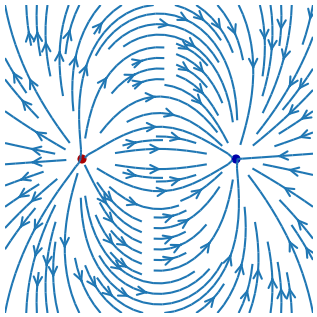
\includegraphics[width=0.3\textwidth]{figures/electric_field.png}
	\caption{Electric field around two opposing charges.}
	\label{fig:electric-field}
\end{wrapfigure}

Electromagnetism can ultimately thought of as the interaction between positively and negatively charged particles.
Charged particles are attracted to other particles of the opposite charge, and repelled by like charge.
Force exerted between two oppositely charged particles effects a region of space where other charges will be affected.
This is called an electric field and can be seen in Figure \ref{fig:electric-field} as depicted with field lines, where the arrows indicate the direction of the force experienced by a positive test charge.
The magnitude of the electric field at some point in space, as experienced by a positive test charge, is called the electric field strength, denoted $\bvec{E}$.
Generally, the field strength of an electric field is greater when it is closer to a charge.\footcite{britelectric}

\newpage

\begin{wrapfigure}[11]{r}{0.3\textwidth}
	\centering
	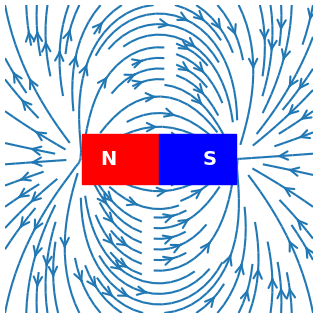
\includegraphics[width=0.3\textwidth]{figures/magnet_field.png}
	\caption{Magnetic field around a magnetic dipole.}
	\label{fig:magnet-field}
\end{wrapfigure}

In terms of magnetism, magnets embody this principle by having two poles, north and south, which could be thought of as positive and negative poles respectively.
In this way, opposite poles attract while like poles repel.
The region in which a magnetic dipole is effected by these forces is called a magnetic field and is depicted in Figure \ref{fig:magnet-field}.
The field lines of a magnetic field point from north to south.
There are two nearly identical vector fields that represent a magnetic field; magnetic field strength, $\bvec{H}$ or H-field, and magnetic flux density, $\bvec{B}$ or B-field.
While their differences are beyond the scope of this investigation, it is important to know that an H-field is concerned with the field strength of a specific point while a B-field is concerned with the density of the field lines at a specific point, also known as flux density.
This investigation concerns the latter field, magnetic flux density, and will refer to it as a magnetic field.\footcite{britfields}

Electricity also embodies this principle in electric current, where negatively charged electrons flow towards a more positive charge.
However, conventional thinking would have the direction of current as the movement from higher to lower charge, hence current flows from positive to negative.
This movement of charge is what creates magnetic fields.
Specifically, if current is moving through a wire, than the movement of charge creates a magnetic field whose field lines are concentric circles around the wire, perpendicular to the direction of current.\footcite{msufields}
Similar to how magnets can attract or repel each other, these moving charges are also subject to magnetic force.
This force, combined with electric force, is called Lorentz force.

\subsection*{Lorentz Force}

\begin{wrapfigure}[10]{r}{0.3\textwidth}
	\centering
	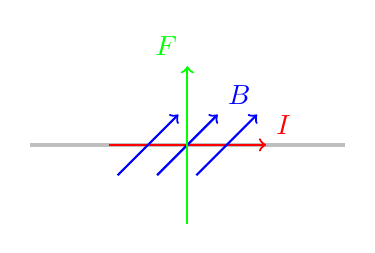
\begin{tikzpicture}
		\draw[ultra thick,lightgray] (-2,0,0) -- (2,0,0);
		\draw[thick,red,->] (-1,0,0) -- (1,0,0) node[above right]{$I$};
		\draw[thick,blue,->] (-0.5,0,1) -- (-0.5,0,-1);
		\draw[thick,blue,->] (0,0,1) -- (0,0,-1) node[above right]{$\bvec{B}$};
		\draw[thick,blue,->] (0.5,0,1) -- (0.5,0,-1);
		\draw[thick,green,->] (0,-1,0) -- (0,1,0) node[above left]{$\bvec{F}$};
	\end{tikzpicture}
	\caption{Force on a current-carrying wire.}
	\label{fig:laplace-force}
\end{wrapfigure}

Lorentz force, in terms of vectors, is defined as:
\begin{equation*}
	\bvec{F} = q\bvec{E} + q\bvec{v} \times \bvec{B}
\end{equation*}
where $q$ is the charge of a point particle, $\bvec{v}$ is the velocity of the particle, $\bvec{E}$ is the electric field, and $\bvec{B}$ is the magnetic field.
This equation represents the forces experienced by a charged particle in an electromagnetic field.
The cross product of $\bvec{v}$ and $\bvec{B}$ indicates that the force is perpendicular to both the direction of velocity and the magnetic field.\footcite{navelorentz}

\newpage

Lorentz force can be extended to describe the relationship between magnetic force and a current-carrying wire.
If the wire is placed in a uniform magnetic field with no electric field, then the equation simplifies to:
\begin{equation*}
	\bvec{F} = q\bvec{v} \times \bvec{B} \text{.}
\end{equation*}
Knowing that $\bvec{v}$ is the length of the wire $\bvec{L}$ divided by time $t$, and that current $I$ is the number of charged particles going through a point over time, the equation can then be rewritten to:\footcite{navelaplace}
\begin{align*}
	\bvec{F} &= q\frac{\bvec{L}}{t} \times \bvec{B} \\
	\bvec{F} &= \frac{q}{t}\bvec{L} \times \bvec{B} \\
	\bvec{F} &= I\bvec{L} \times \bvec{B} \text{.}
\end{align*}
This force is illustrated in Figure \ref{fig:laplace-force}, where current, B-field, and force are all perpendicular to each other.
Assuming that the current, B-field, and force are perpendicular to begin with, then the equation can be written as:
\begin{equation}
	F = ILB \label{eqn:laplace}
\end{equation}

\subsection*{Experimental Equation}

In order to test this relationship, an elements of Lorentz force must be used as the independent and dependent variables.
For the dependent variable, force is the most flexible variable to measure.
As for the independent variable, there are three options.
Looking at Equation \eqref{eqn:laplace}, of current, length, and B-field strength, current is the easiest to vary.
For B-field strength, either the type of magnet would be varied at the same distance from the wire, or the distance would be varied, of which the latter will be much more difficult since a magnetic field does not completely adhere to the inverse square law.\footcite{wwdistance}
As for length, a magnet would be required whose surface area could cover the range test lengths.
Current, on the other hand, can easily be varied by varying the voltage output of a power supply.
However, current should be limited to under two amps to reduce the chance of burns, whether it be electrical or heat emitted by components.
This means that force will inherently be quite small, even if its magnitude is scaled by using strong magnets.

In order to measure a small force, a pendulum apparatus similar to the CGI video demonstration by the National High Magnetic Field Laboratory will be used.\footcite{nmllorentz}
The deflection angle can be used to determine the Lorentz force through vector analysis.
Letting $\theta$ represent the deflection angle and $F$ represent the Lorentz force, the relationship between both variables is defined as:
\begin{equation}
	F = mg \tan\theta \text{.} \label{eqn:experiment}
\end{equation}
Thus, $F$ is proportional to $\tan\theta$.
